\documentclass[12pt]{article}
 
\newenvironment{sol}[1][Solution]{\begin{trivlist}\item[\hskip\labelsep {\bfseries #1:}]}{\end{trivlist}}
\usepackage{minted}
%\usemintedstyle{perldoc}
\usemintedstyle{vs}
\usepackage{graphicx}
\graphicspath{./}

\usepackage[margin=1in]{geometry} 
\usepackage{amsmath,amsthm,amssymb}
\usepackage{times,url}
\usepackage{tikz}
\usepackage{color}
\usepackage{enumerate}
\begin{document}
\renewcommand{\qedsymbol}{\filledbox}
\begin{center}
    \textbf{CS 5/7350 - Test\#3} \\
    \textbf{Fall, 2021}
%replace X with the appropriate number
\end{center}
\begin{flushright}
Name: \underline{Bingying Liang }\\
ID:  \underline{\ \ \ \ \ 48999397 \ \ \ \ \ }
\end{flushright}
\begin{enumerate}
    \item \ [5 pts] The following numbers are in the number system $\beta= \frac{1}{\sqrt[3]{2}}$ (one over the cube root 3
of 2) and D = \{0,1\}. Add the numbers and give the answer in the same number system:
\begin{sol}
\hspace*{\fill}
            \begin{center}
    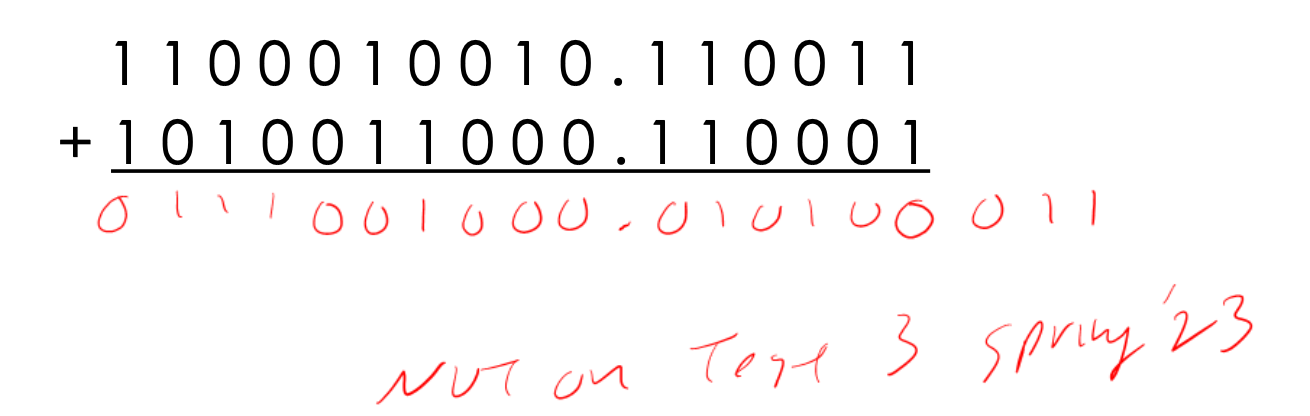
\includegraphics[width=0.6\textwidth]{p1.png}
    \end{center} 
\end{sol}

\item \ [8 pts] You want to prove that some problem H is NP-Complete. You know that problem G is NP-Hard. Mark \textbf{True} for each of the following statements of things you need to prove. Mark \textbf{False} if you do not need to prove the statement.
    \begin{enumerate}
        \item You need to prove that H can be verified in polynomial time.
        \begin{sol}
            True
        \end{sol}
        \item You need to prove that G can be verified in polynomial time.
        \begin{sol}
            False
        \end{sol}
        \item \textcolor{red}{You need to prove that a solver for G can also solve H.}
        \begin{sol}
            False
        \end{sol}
        \item \textcolor{red}{You need to prove that a solver for H can also solve G.}
        \begin{sol}
            True
        \end{sol}
        \item You need to prove that H is NP-Hard
        \begin{sol}
            True
        \end{sol}
    \end{enumerate}

    \item \ [7 pts] Compute the integer value for Z given that ( (161 * Z) + 3879 ) modulo 11609 = 11169. Show your table for the Extended Euclidian Algorithm.
 \begin{sol}
    \begin{align*}
        & (161 \times Z + 3879) \bmod 11609 = 11169 \\
        & (161 \times Z) \bmod 11609 + 3879 \bmod 11609 = 11169 \\
        & (161 \times Z) \bmod 11609 + 3879 = 11169 \\
        & (161 \times Z) \bmod 11609 = 7290 \\ 
        & (161 \times Z) \bmod 11609 = 7290 \bmod 11609 \\ 
        & (\frac{1}{161}\times 161 \times Z) \bmod 11609 = (\frac{1}{161} \bmod 11609) \times (7290 \bmod 11609)\\
        & Z \bmod 11609 = (\frac{1}{161} \bmod 11609) \times (7290 \bmod 11609) \\
    \end{align*}
    \begin{center}
        \begin{tabular}{|c|c|c|c|c|c|c|}
        \hline
             & A & B & Q & R & $\alpha$ & $\beta$   \\
             \hline
        -1   &   &   &   &   &      1    &  0 \\
        \hline
        0    & 11609  &  161  & 72   & 17   &      0    &  1 \\
        \hline
        1    & 161   &  17  & 9 & 8 & 1 & -72 \\
        \hline
        2 & 17 & 8 & 2  & 1 & -9 & 649 \\
        \hline
        3 & 8 & 1 & 8 & 0 & 19 & -1370 \\
        \hline
        4 & 1 & 0 & - & - & -161 & 11609 \\
        \hline
        \end{tabular}
        \begin{align*}
            & 19 \times 11609 = 220571\\
            & 1370 \times 161 = 220570\\
            & 19 \times 11609 - 1370 \times 161 = 1\\
            & (19 \times 11609) \bmod 11609 - (1370 \times 161) \bmod 11609 =  1 \bmod 11609\\
            & 0+ (-1370 \times 161) \bmod 11609 = 1  \\
             & (- 1370 \times 161) \bmod 11609 = 1\\
            & (\frac{1}{161}) \times 161 \bmod 11609 = 1 \\ 
            & \therefore (\frac{1}{161})\bmod 11609 = (-1370) \bmod 11609\\
            & (\frac{1}{161} \bmod 11609) = (11609 - 1370) \bmod 11609\\
            & (\frac{1}{161}) \bmod 11609 = 102309 \bmod 11609\\
            & \therefore Z \bmod 11609 = 102309 \times (7290 \bmod 11609) \\
            & Z \bmod 11609 = (102309 \times 7290) \bmod 11609\\
            & Z \bmod 11609 = 8049\\
            & \therefore Z = 11609i + 8049, \text{where i is an integer}.
        \end{align*}
    \end{center}
    \end{sol}

    \item \ [6 pts] Show the addition table required for addition that adds two numbers from the number system $\beta$= 7 and D = \{ -4 -3, -2, -1, 0, 1, 2, 3, 4 \} giving a number in the same number system. Ensure the addition can be performed in parallel without having to “ripple” a carry. (You do not need to fill in the grey areas:
    \begin{sol}
    \hspace*{\fill}
            \begin{center}
    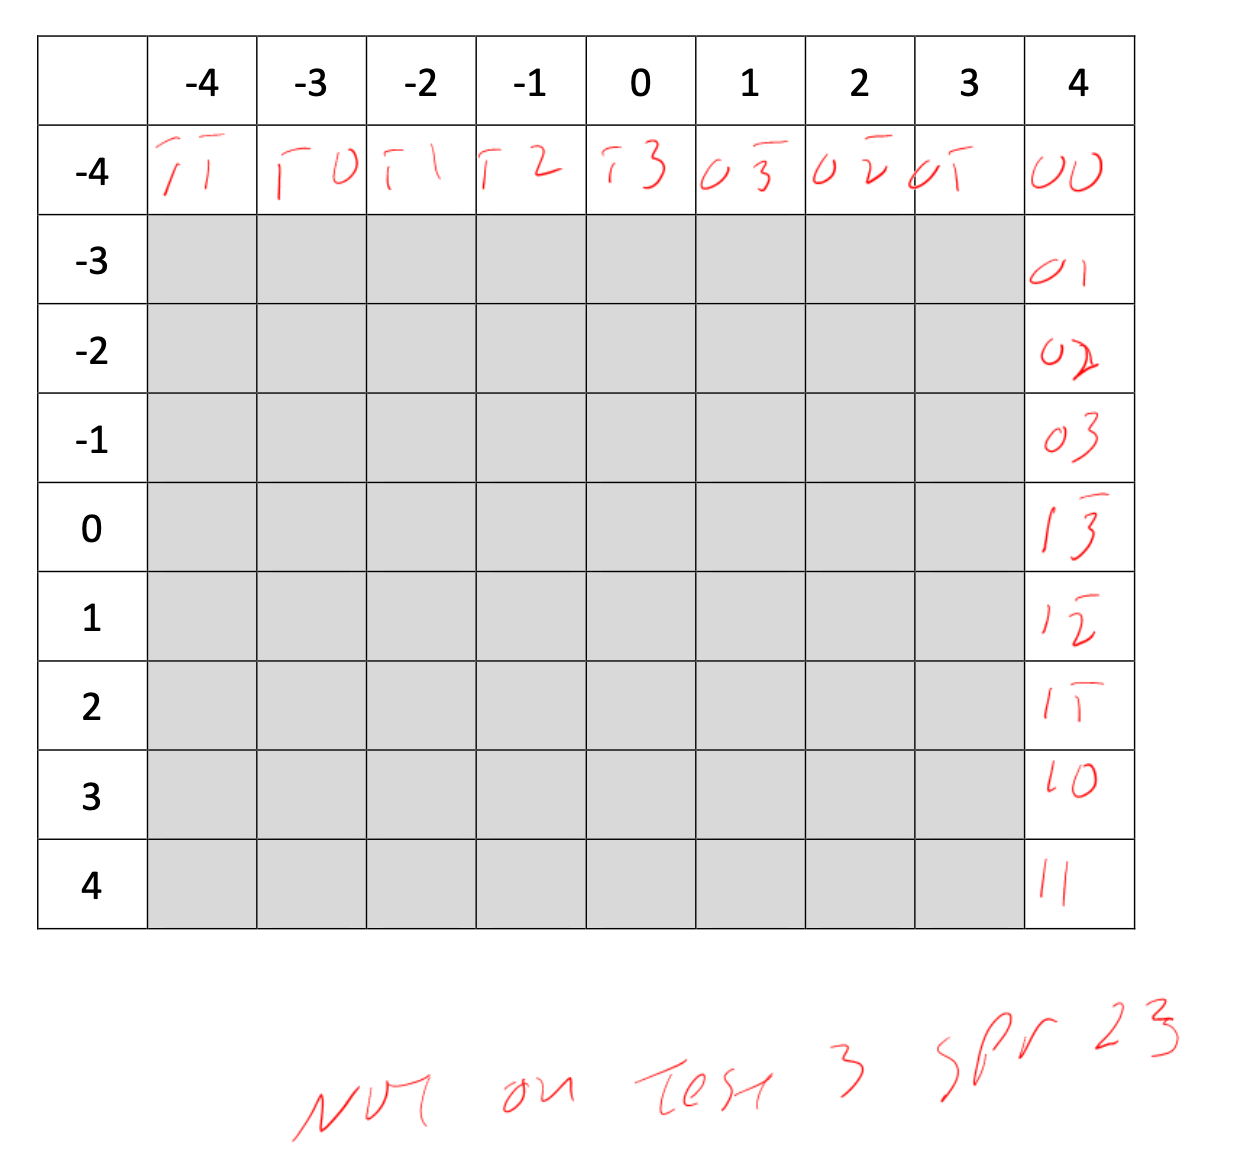
\includegraphics[width=0.6\textwidth]{p2.png}
    \end{center} 
\end{sol}
    
    \item \ [8 pts] You have 3 dice. Each one is different.
    \begin{itemize}
        \item Die \#1 has sides \{ 0, 1, 2 \} with a
        \begin{itemize}
            \item 20\% chance of rolling a 0, a
            \item 30\% chance of rolling a 1 and a
            \item 50\% chance of rolling a 2.
        \end{itemize}
        \item Die \#2 has sides \{ 2, 2, 0 \} with a
        \begin{itemize}
            \item 35\% chance of rolling the first 2 and a
            \item 35\% chance of rolling the other 2 and a
            \item 30\% chance of rolling a 0
        \end{itemize}

        \item Die \#3 has sides \{0, 1\} with a
        \begin{itemize}
            \item 25\% chance of rolling a 0 and a
            \item 75\% chance of rolling a 1
        \end{itemize}
    \end{itemize}
    \begin{enumerate}
        \item Fill in the table for the dynamic programming algorithm to solve the problem.
        \begin{sol}
        \hspace*{\fill}
                                    \begin{center}
    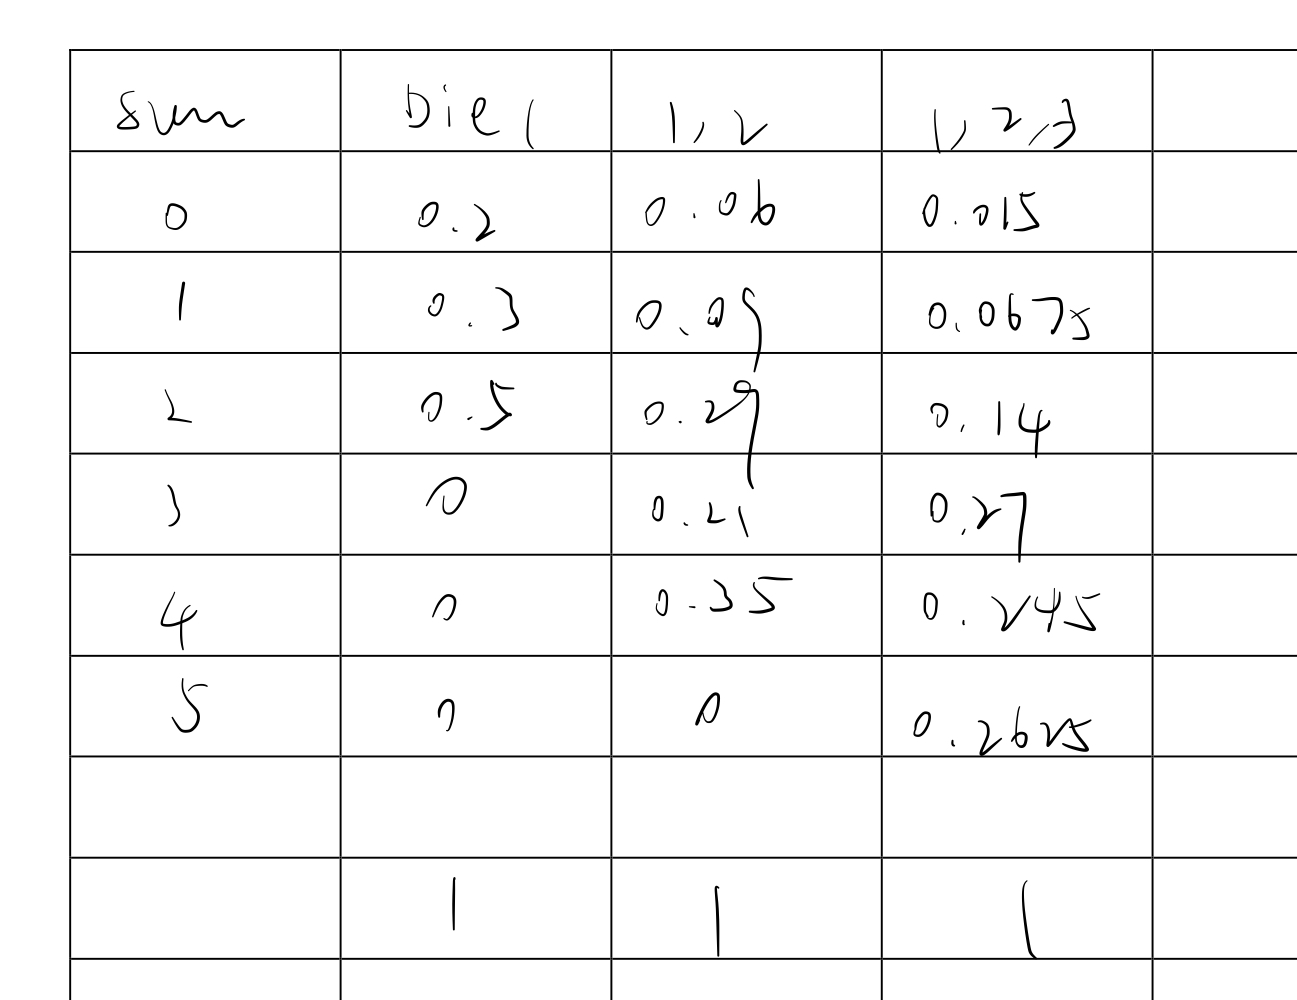
\includegraphics[width=0.4\textwidth]{p3.jpeg}
    \end{center} 
        \end{sol}
        \item What is the probability of rolling a 0?
        \begin{sol}
            0.015
        \end{sol}
        \item What is the probability of rolling a 1?
                \begin{sol}
            0.9675
        \end{sol}
        \item What is the probability of rolling a 2?
                \begin{sol}
            0.14
        \end{sol}
        \item What is the probability of rolling a 3?
                \begin{sol}
            0.27
        \end{sol}
        \item What is the probability of rolling a 4?
                \begin{sol}
            0.245
        \end{sol}
        \item What is the probability of rolling a 5?
                \begin{sol}
            0.2625
        \end{sol}
    \end{enumerate}

    \item \ [8 pts] Create a graph with a starting vertex of “S” (when required) where:
    \begin{enumerate}
        \item The weight of the third edge chosen with Prims Minimum Spanning Tree Algorithm is less than the weight of the third edge chosen with Kruskal’s Minimum Spanning Tree Algorithm. Mark the third edge chosen by prim’s algorithm with a “P” and the third edge chosen by Kruskal’s algorithm with a “K”.
                \begin{sol}
        \hspace*{\fill}
                                    \begin{center}
    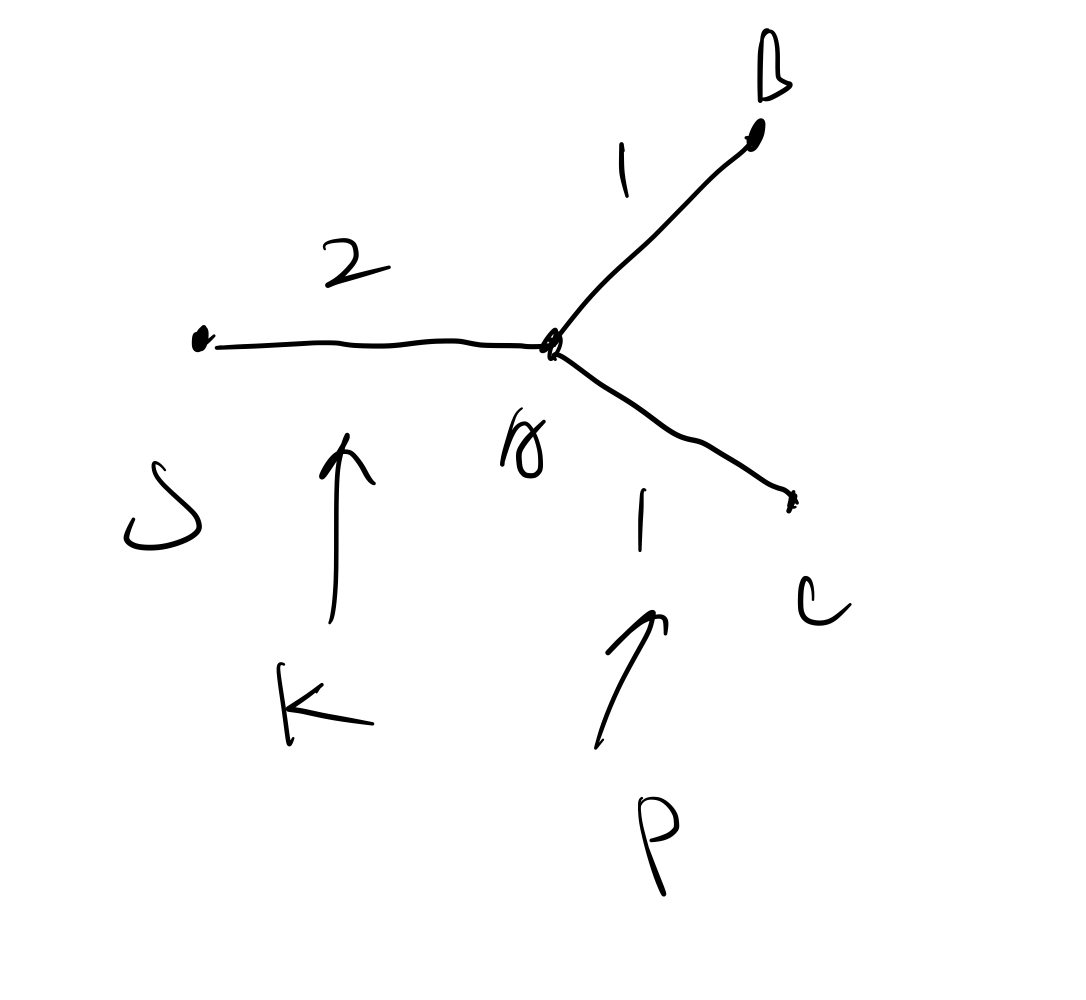
\includegraphics[width=0.3\textwidth]{p7.jpeg}
    \end{center} 
        \end{sol}
\item The weight of the third edge chosen with Kruskal’s Minimum Spanning Tree Algorithm is less than the weight of the third edge chosen with Prims Minimum Spanning Tree Algorithm. Mark the third edge chosen by prim’s algorithm with a “P” and the third edge chosen by Kruskal’s algorithm with a “K”.
        \begin{sol}
        \hspace*{\fill}
                                    \begin{center}
    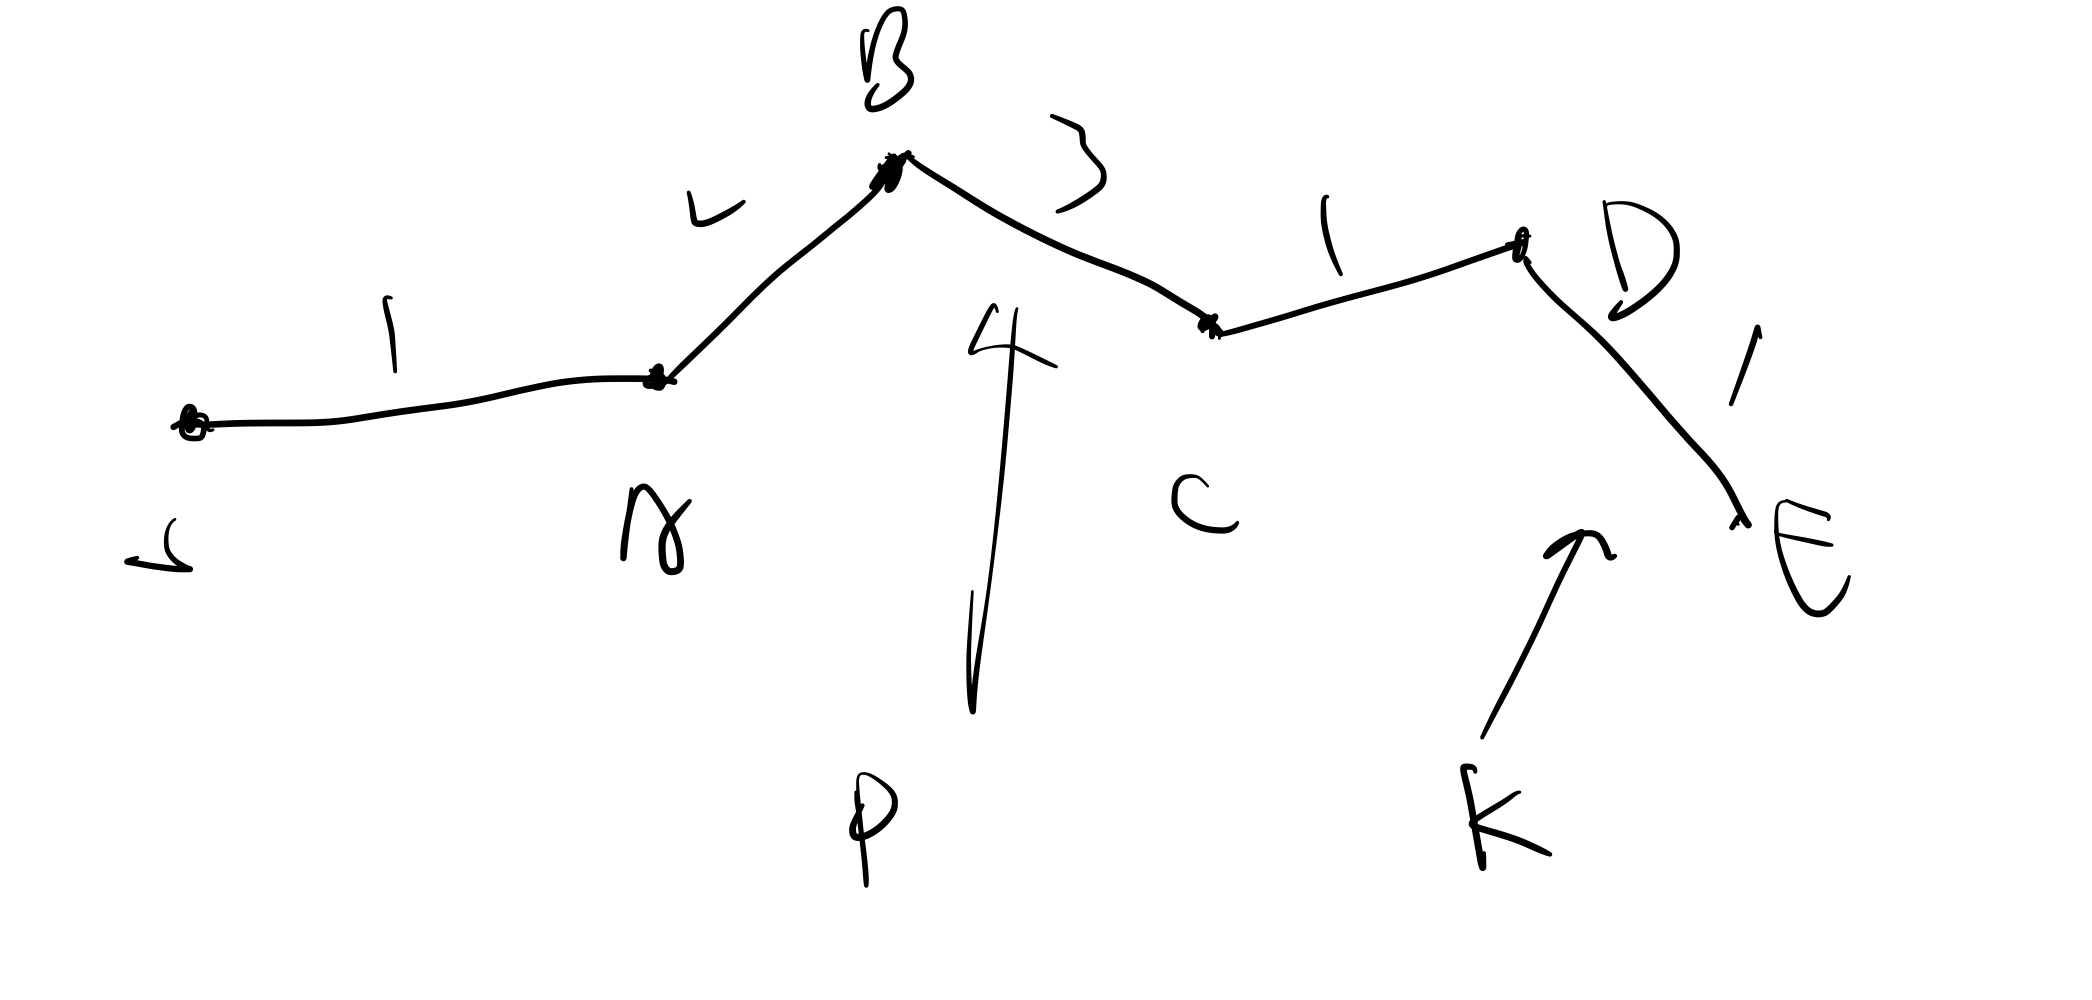
\includegraphics[width=0.4\textwidth]{p8.jpeg}
    \end{center} 
        \end{sol}
    \end{enumerate}


    \item \ [8 pts] Answer the following questions.:
    \begin{enumerate}
        \item A program requires 3s to brute force attack an encryption key of 64 bits. If the
running time is $\Theta(2^n)$ about how many years would it take to brute force attack an encryption key of 256 bits? (note there are about 32 million seconds in a year)
\begin{sol}
    $2^{192} \times 3 \times \frac{1}{32\times 10^6}s$
\end{sol}
\item A program requires 3s to brute force attack an encryption key of 64 bits. If you have access to a quantum computer where the running time is $\Theta(n^2)$ about how many seconds would it take to brute force attack an encryption key of 256 bits?
\begin{sol}
    48s
\end{sol}

    \end{enumerate}

    \item \ [7 pts] Use the DGT algorithm discussed in class to determine how to represent the value 282 using the number system $\beta$=5, D = \{ -2, -1, 0, 7 \}. Show your work.
    \begin{sol}
        \begin{align*}
            & -2 \bmod 5 = 3, -1 \bmod 5 = 4, 7 \bmod 5 = 2\\ 
            & 282 \bmod 5 = 2 \rightarrow 7\\
            & 282-7 = 275 \\
            & 275 \div 5 = 55\\
            & ---------------\\
            & 55 \bmod 5 = 0\\
            & 55 - 0 = 55\\
            & 55 \div 5 = 11 \\
            & ---------------\\
            & 11 \div 5 = 1 \rightarrow No \ digit \ is =1.\\
            &\therefore 282 \text{can not be represented in this number system}
        \end{align*}
    \end{sol}

    \item \ [7 pts] A tree has the following pre-order and in-order traversals. Draw the tree and give the post-order traversal.
    \begin{center}
        In-Order: GFIHABDKCEJ \\
        Pre-Order: AFGHICDBKEJ   
    \end{center}
        \begin{sol}
        \hspace*{\fill}
    \begin{center}
    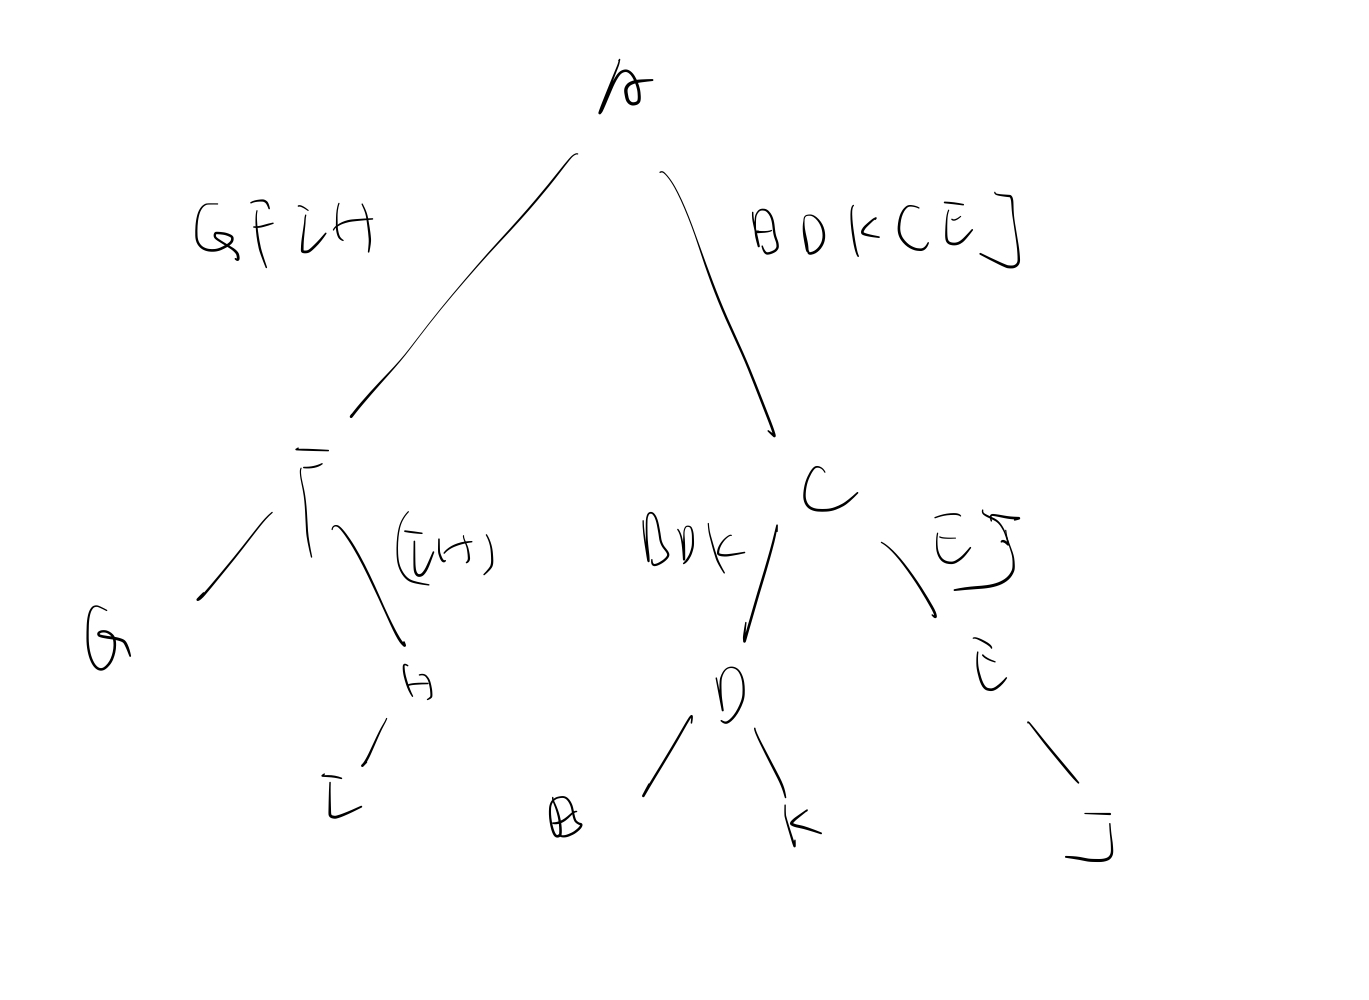
\includegraphics[width=0.6\textwidth]{p4.jpeg}
    \end{center} 
    \end{sol}

    \item \ [8 pts] You have two strings, A and B.
\begin{itemize}
    \item String A has a length of 8.
    \item String B has an unknown length.
    \item The Lowenstein Edit Distance between the two strings is 5.
\end{itemize}
\begin{enumerate}
    \item What is the minimum length of String B?
    \begin{sol}
        3
    \end{sol}
    \item What is the maximum length of String B?
    \begin{sol}
        13
    \end{sol}
    \item What is the minimum length of the Longest Common Subsequence of String A and String B
    \begin{sol}
        3
    \end{sol}
    \item \textcolor{red}{What is the maximum length of the Longest Common Subsequence of String A and String B?}
    \begin{sol}
        8
    \end{sol}

\end{enumerate}

\item \ [8 pts] You run different programs for various values of “n” and sometimes “m” and create 4 tables of the runtimes. Give the asymptotic bounds that each table supports?
    \begin{center}
    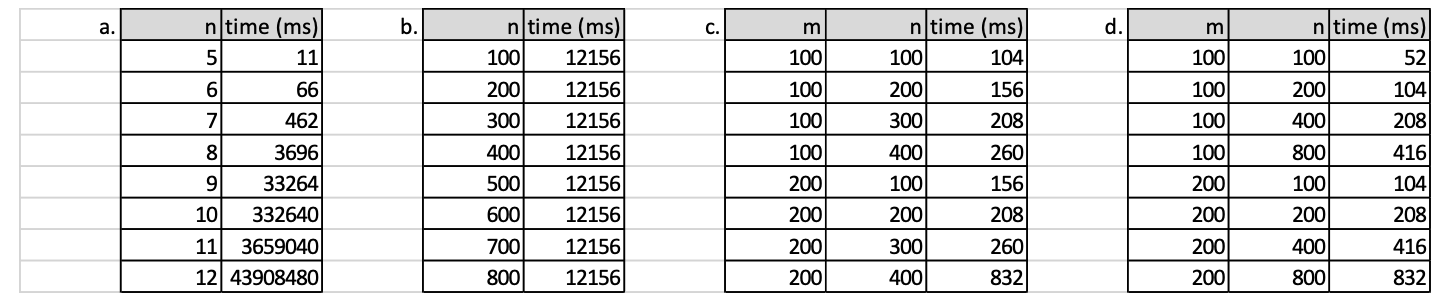
\includegraphics[width=0.9\textwidth]{p5.png}
    \end{center} 
    \begin{sol}
    \hspace*{\fill}
        \begin{enumerate}
            \item $\Theta(n!)$
            \item $\Theta(1)$
            \item $\Theta(n+m)$
            \item $\Theta(mn)$
        \end{enumerate}
    \end{sol}


    \item \ [6 pts] Two people need to establish a secret key for encrypting communications. They agree to use a Diffie-Hellman key exchange with a modulus of 13 and decide on 2 as the base. Person A chooses a random value of 4 and person B chooses a random value of 9.
    \begin{enumerate}
        \item What is the value Person A sends to Person B
        \begin{sol}
            3
        \end{sol}
        \item What is the value Person B sends to Person A
        \begin{sol}
            5
        \end{sol}
        \item What is the shared secret key between Person A and Person B
        \begin{sol}
            1
        \end{sol}

    \end{enumerate}
    \item \ [6 pts] Using $n_0$ equal to 10, determine the maximum value for $c_1$ and the minimum value for c2, required to show that $f(n) = 7n^2 + 3n + 5$ is $\Theta(n^2)$.
        \begin{sol}
        \begin{align*}
            \Omega(n^2): & 0 \leq c_1g(n) \leq f(n), \forall n = n_0 = 10\\
            & c_1 n^2 \leq 7n^2 + 3n + 5, \forall n = n_0 = 10\\
            & c_1 \leq 7 + \frac{3}{n} + \frac{5}{n^2}, \forall n = n_0 = 10\\
            & c_1 \leq 7 + \frac{3}{10} + \frac{5}{10^2}\\
            & \therefore c_1 = 7 \text{ can let }f(n) \text{ is } \Omega(n^2), \forall n = n_0 = 10
        \end{align*}
                \begin{align*}
            O(n^2): & 0 \leq  f(n)\leq c_2g(n), \forall n = n_0 = 10\\
            & 7n^2 + 3n + 5 \leq c_2 n^2, \forall n = n_0 = 10\\
            & 7 + \frac{3}{n} + \frac{5}{n^2} \leq  c_2 , \forall n = n_0 = 10\\
            & 7 + \frac{3}{10} + \frac{5}{10^2} \leq  c_2\\
            & 7.35 \leq c_2 \\
            & \therefore c_2 = 7.35 \text{ can let }f(n) \text{ is } O(n^2), \forall n = n_0 = 10 \\
        \end{align*}
    \end{sol}

    \item \ [8 pts] Determine a Huffman encoding for each symbol in a message that contains:
    \begin{center}
        20 A's, 7 B's, 7 C's, 5 D's, 2 E's and 2 F's.
    \end{center}
    \begin{enumerate}
        \item How many bits are in the entire message if each symbol is encoded with 3 bits?
        \begin{sol}
            129 bits
        \end{sol}
        \item How many bits are in the entire Huffman coded message?
        \begin{sol}
            93 bits
        \end{sol}
        \item How much entropy does each “B” have in the message?
        \begin{sol}
            $\log_2(\frac{43}{7})$ bits
        \end{sol}
            \begin{center}
    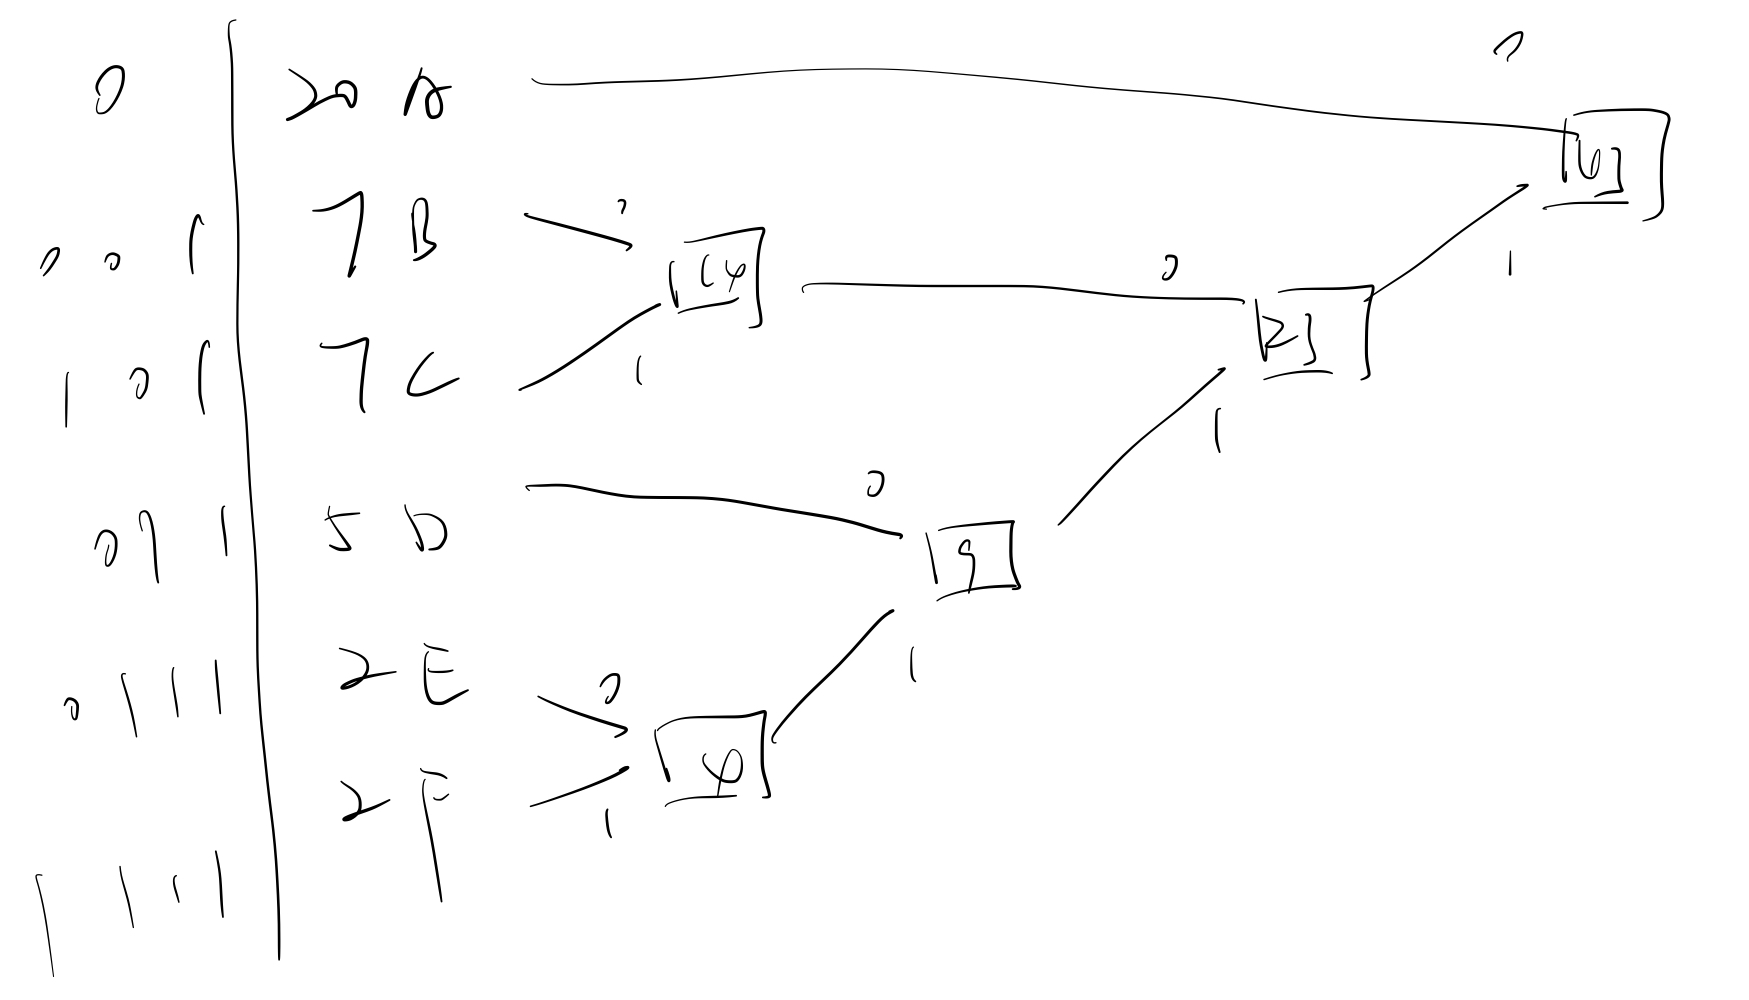
\includegraphics[width=0.6\textwidth]{p6.jpeg}
    \end{center} 
    \end{enumerate}



\end{enumerate}
\end{document}
